\section{Experiments}
\subsection{Simulated Data}
For each experiment a diploid population is created and evolved as follows. 
\paragraph{I. Creating initial founder lines}
First using msms prgram, we created a population for $F$ founding haplotypes with parameters \texttt{\$./msms <F> 1 -t <4μLNe> -r <4Ne(L − 1)r> <L>} where $F=200$ is number of founder lines, 
$L=10^5$, $\theta=4\mu LNe=17$ and $\rho=4Ne(L-1)r=4$.  (assuming $Ne=1000$, $r=10^{-8}$ and $\mu=4.25\times 10^{-8}$).  
\paragraph{II. Creating initial diploid population} 
To mimic the real E\&R experiment for diploid organisms, first initial haplotypes cloned to create $F$ diploid homozygotes. Then each diploid is cloned $N/F$ times to yield $N$ diploid homozygote organisms.
\paragraph{III. Forward Simulation}
Given initial diploid population, position of the site under selection, selection strength $s$, number of replicates $R=3$, recombination rate $r=10^{-8}$ and sampling times $\Tc$ simuPop is used to perform forward simulation and compute allele frequencies for all of the $R$.

\begin{figure}[H]
  \centering
  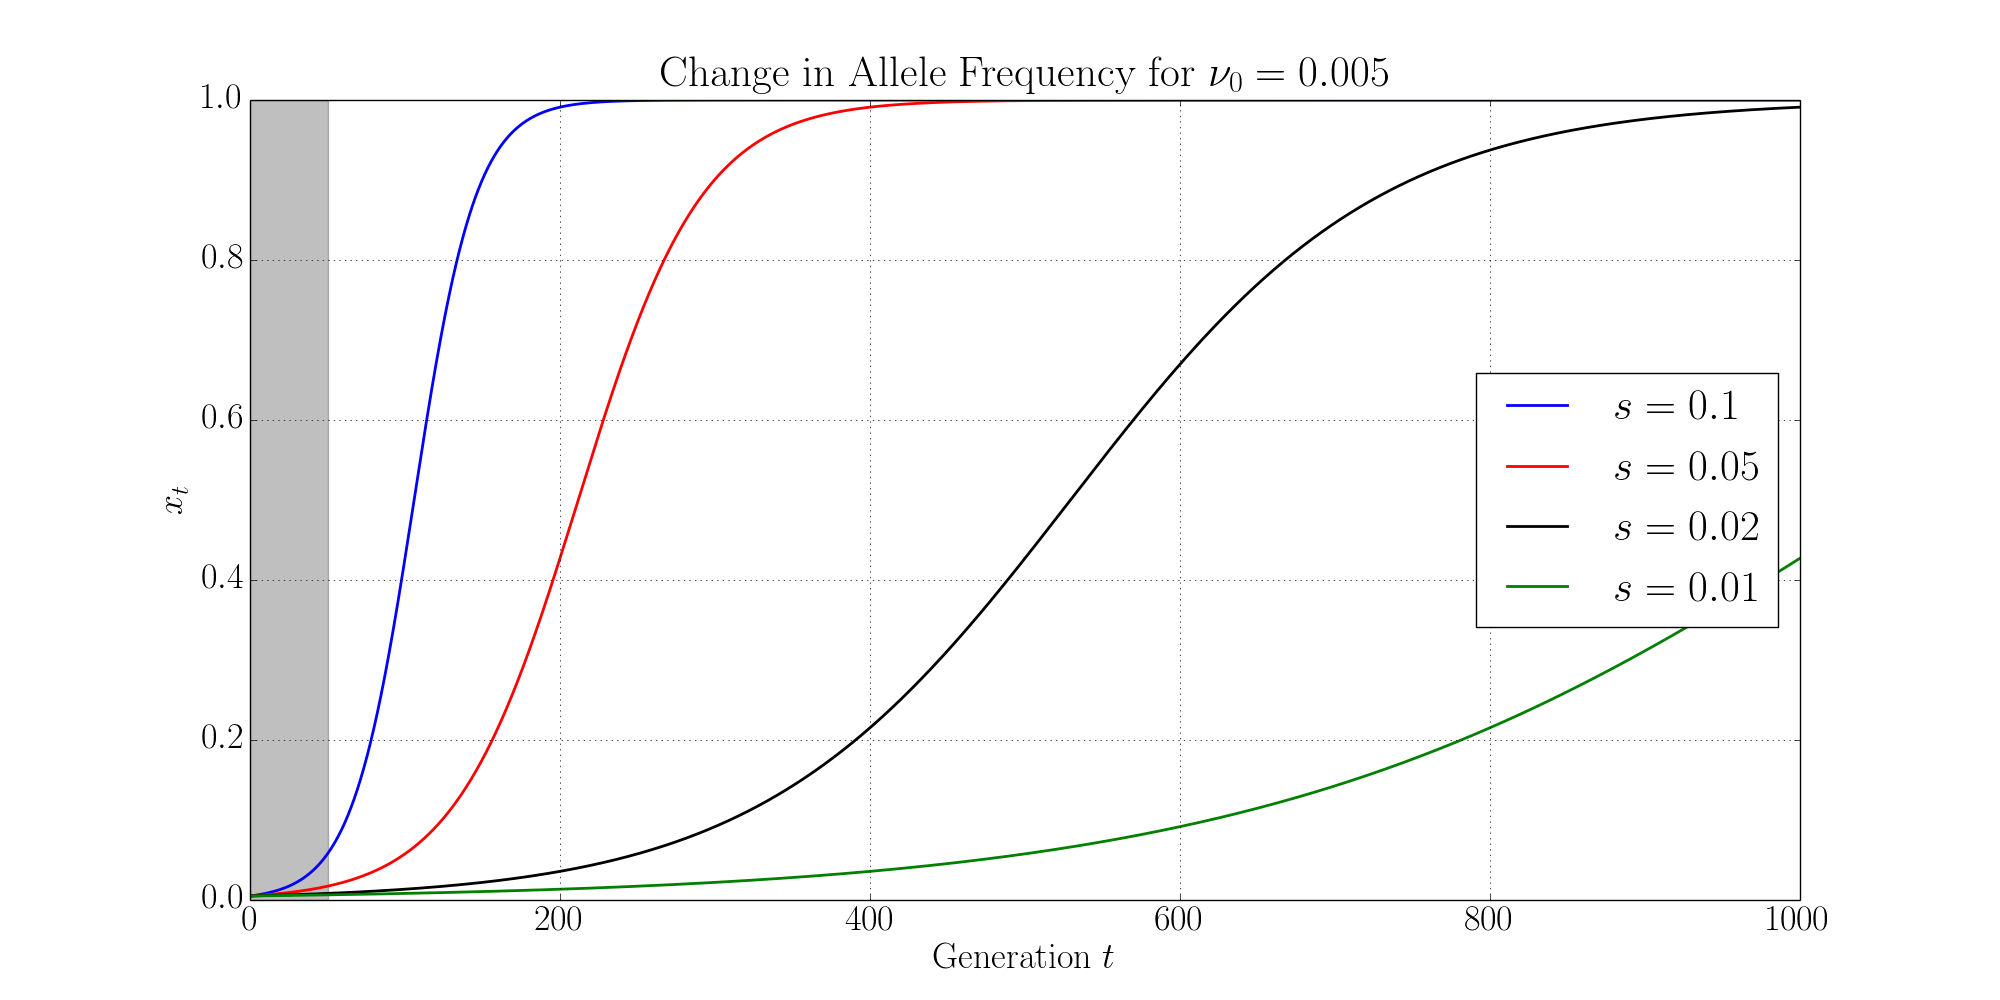
\includegraphics[trim={ 2in 0 1.8in 0},clip,scale=0.4]{sigmoidHard.png}
\end{figure}

\subsection{Sampling Times}
$\Tc=\{0,10,20,\ldots ,100\} + \delta$ where $\delta$ is randomly chosen so that sampling is taken up along different epochs of sweep for different experiments.
we van rearrange \eqref{naive2point}
\beq
t=\frac{2}{s}(\nu(x_t)-\nu(x_0))
\eeq
where setting $x_t=1/2$, we can compute fixatoin time 
\beq
t_{Fix}=\frac{-4\eta(x_0)}{s}
\eeq
In the case of hard sweep, by setting fixation frequency to $x_t=1-1/F$ and $x_0=1/F$ time to fixation can be computed
\beq
\eta(1-1/F)=st/2+\eta(1/F)\\
t_{Fix}(s)=2\frac{\eta(1-1/F)-\eta(1/F)}{s}=\frac{-4\eta(1/F)}{s}
\eeq
To emphasize on mid frequency samples, we sample with rejection from discrete normal $\Nc_d$ with $\mu=t_{Fix}(s)/2$, i.e., time to $x_t=0.5$ and std of $t_{Fix}(s)/6$ (so that $[0,t_{Fix}]=[\mu-3std, \mu+3std]$ be the 99.5\% confidence interval).
\beq
\delta \sim \Nc_d(t_{Fix}/2, t_{Fix}/4)
\eeq
\subsection{Detecting Selection}

\subsubsection{Hard Sweep}
\begin{table}
  \begin{center}
    \begin{tabular}{l|c|c}
Method&AUC&Approach \\
\hline
FayWu`s  H&0.9241&MultiLocus \\
FayWu`s  H-Classic&0.5575&MultiLocus \\
HAF&0.9798&MultiLocus \\
SFSelect&0.9895&MultiLocus \\
 \bf{SFSelect-Classic}& \bf{0.9904}& \bf{MultiLocus} \\
Tajima`s  D&0.9773&MultiLocus \\
Tajima`s  D-Classic&0.9791&MultiLocus \\
Gaussian  Process&0.9251&SingleLocus \\
Least  Squares&0.8495&SingleLocus \\
Naive&0.8769&SingleLocus \\
Naive-Classic&0.9824&SingleLocus \\
    \end{tabular}
  \end{center}
  \caption{s=0.01}
\end{table}


\subsubsection{Hard Sweep vs Soft Sweep}
\subsubsection{Effects of carrier frequency}
\subsubsection{Effects of sampling times}
\subsubsection{Effects of number of replicates}
\subsubsection{Single-Locus vs Multi-locus}
\subsubsection{Time-series vs single-snapshot}

\subsubsection{Soft Sweep}

\subsection{Locating Selection}

\subsection{Strength of  Selection}






%\subsection{Estimated Frequencies}
%Roughly, estimated frequencies follow sigmoid growth. The exact growth is given by applying the transition function $t$ times.
%\href{http://www.wolframalpha.com/input/?i=dx%2Fdt+%3D+s%2F2+%28x%281-x%29%29+%281%2F%281%2Bsx%29%29}{Writhing the ODE and Solving it gives}%
%\beqn
%  \frac{d\nu_t(s)}{dt} &=\frac{s}{2}\nu_t(s)(1-\nu_t(s))\frac{1}{1+s\nu_t(s)} \\
%  \frac{st}{2}-c&=\log\left(\frac{\nu_t}{(1-\nu_t)^{1+s}}\right)   \label{eq:eactODE}
%\eeqn
%However we can not invert \ref{eq:exactODE} in closed form to get $\nu_t$ in terms of other quantities. In other words, the blue curve in the Figure \ref{fig:sigmoid} left, does not have a closed form inverse. But we can compute exact value of $\nu_t$ (and gradients of objective function w.r.t. $s$ ) in $\Oc(T)$. So no need to approximate even though the error is not significant Figure \ref{fig:sigmoid} Right.
%
%\begin{figure}[H]
%  \centering
%    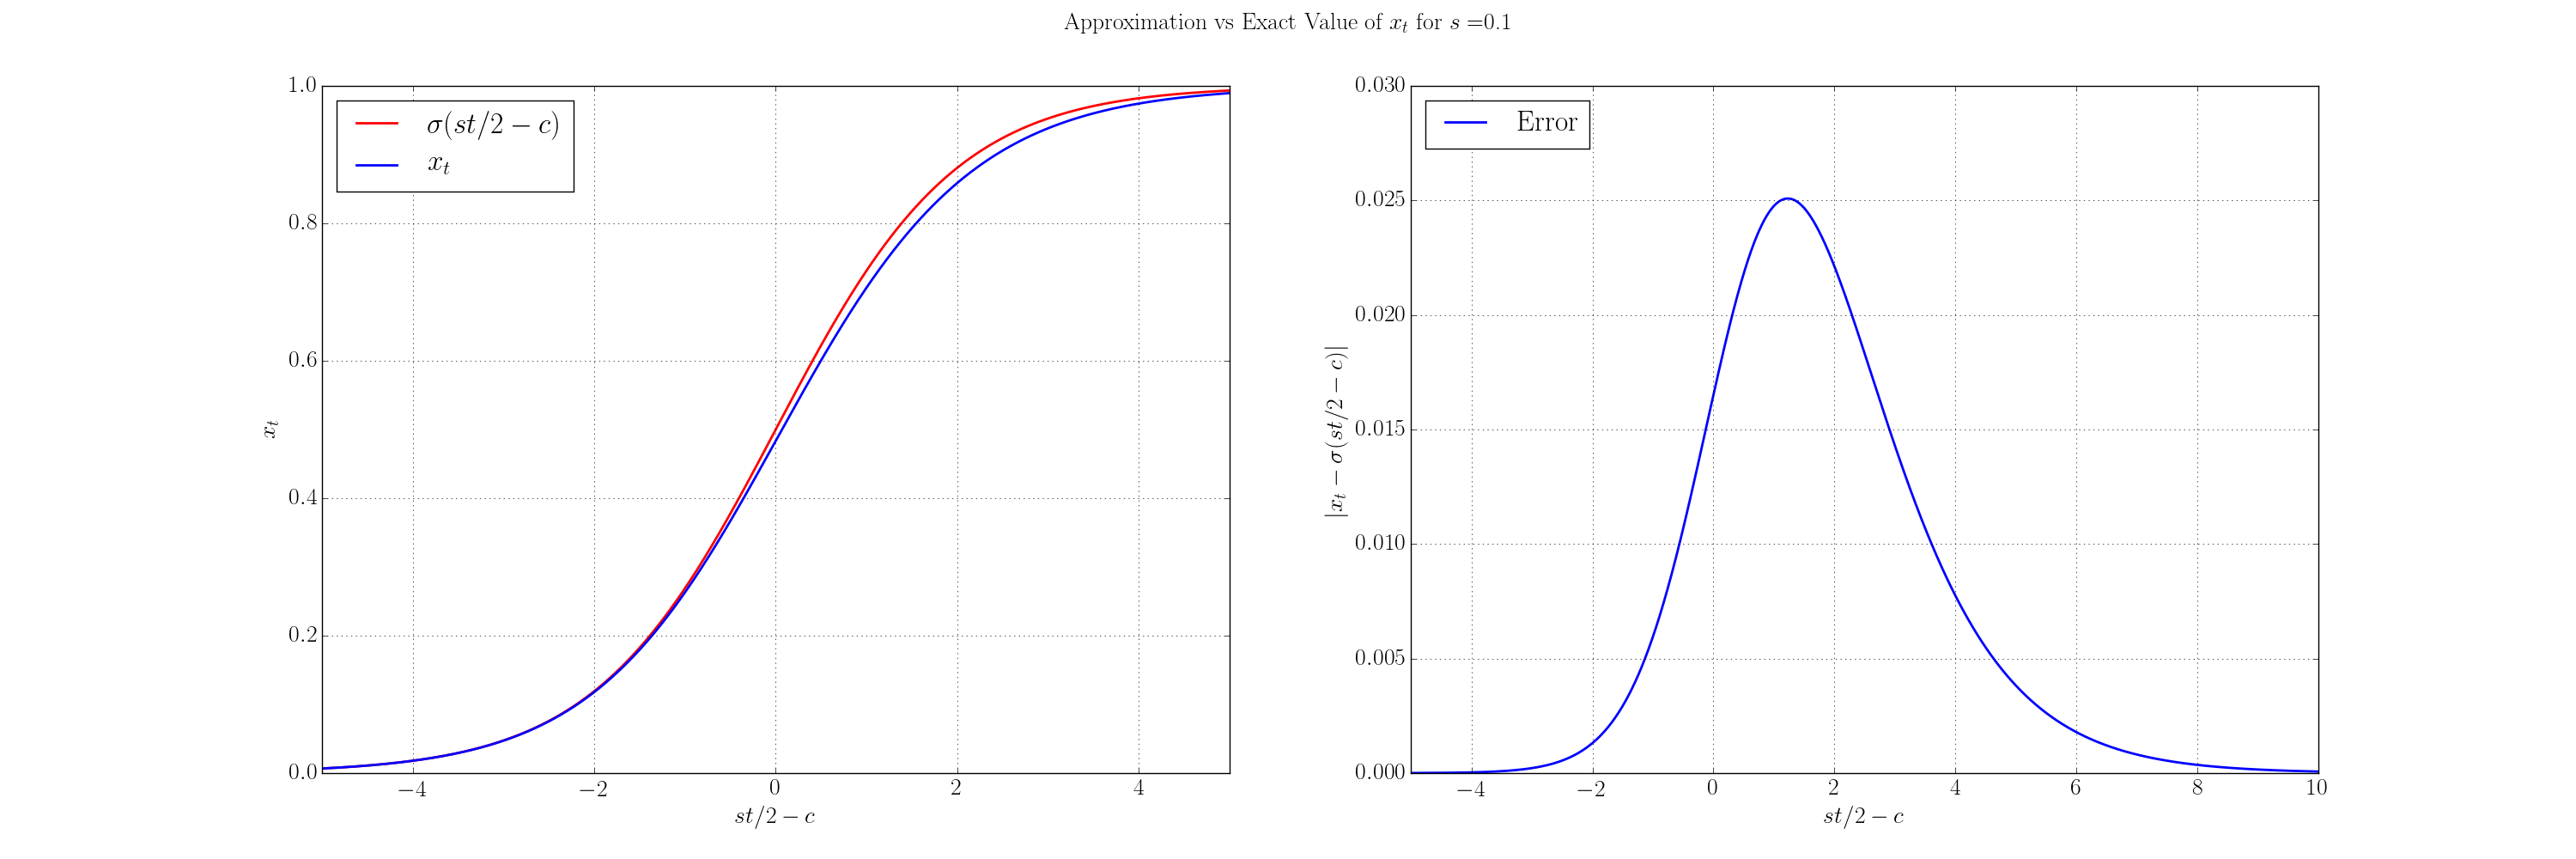
\includegraphics[width=\textwidth]{apprx}
%  \caption{Rank}
%  \label{fig:sigmoid}
%\end{figure}
%
%also $c \approx  \log(F)$ when minor allele is used for selection, i.e., $\nu_0=1/F$
%\subsection{Understanding the difficulty of estimating $s$}
%\subsubsection{Information Theory}
%Signal to Noise Ration(SNR) is high when $s \rightarrow 0$ can be alleviated eliminating noise of genetic drift, i.e.  more replicates. 
%
%\subsubsection{Functional Analysis}
%The slope of sigmoid become close to zero as $s \rightarrow 0$, and can be alleviated by right choice of sampling in time.
